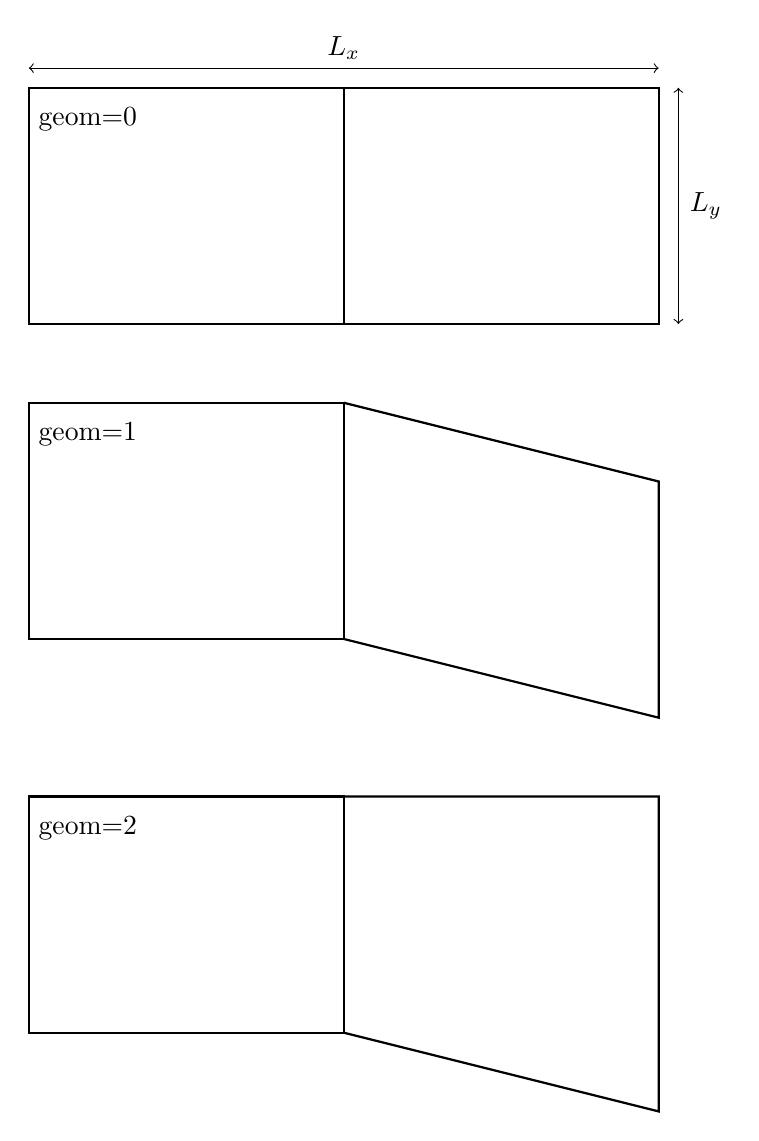
\begin{tikzpicture}
%\draw[step=1cm,gray,very thin] (0,0) grid (10,14); 
\draw[<->,thin] (1,13.25)--(9,13.25);
\node[] at (5,13.5) {$L_x$};
\draw[<->,thin] (9.25,10)--(9.25,13);
\node[] at (9.6,11.5) {$L_y$};
%.............................
\node[] at (1.75,12.6) {geom=$0$};
\draw[thick](1,10) rectangle (5,13); 
\draw[thick](5,10) rectangle (9,13); 
%.............................
\node[] at (1.75,8.6) {geom=$1$};
\draw[thick](1,6) rectangle (5,9);  
\draw[thick](5,6)--(9,5)--(9,8)--(5,9);  
%.............................
\node[] at (1.75,3.6) {geom=$2$};
\draw[thick](1,1) rectangle (5,4);  
\draw[thick](5,1)--(9,0)--(9,4)--(5,4);  
\end{tikzpicture}

